
\section{Simulation and Prediction-Test Fixtures}\label{manual:simulation-prediction-test-fixtures}

\subsection{Scope}\label{manual:simfix:scope}
This manual appendix preserves simulation fixtures and prediction-test placement context downstream from the main note.

\subsection{Statement(s)}\label{manual:simfix:statements}
Required outputs are
\[
RD,
\qquad
\rho^D,
\qquad
\rho^D_\omega,
\qquad
Q^D,
\qquad
p^D,
\qquad
\phi,
\qquad
P^D_F(B),
\qquad
\mathbf A_F(B),
\qquad
\mathcal E(R,B).
\]
Fixtures include
\[
1{:}2{:}6,
\quad
1{:}2{:}7,
\quad
1{:}2{:}8,
\quad
1{:}2{:}9,
\quad
1{:}2{:}10,
\quad
3{:}3{:}6,
\quad
3{:}4{:}6,
\]
\[
3{:}4_\alpha,
\qquad
2\times3{:}4_\alpha,
\qquad
3{:}4_\alpha+3{:}4_\omega.
\]
Separate-scope fixtures include \(3{:}4_\alpha\) and \(3{:}4_\omega\). The fixture set also includes short-window duration-clipping fixture, pending overhang, current split, and AFC Stokes residual.


The nine-window surplus assertion is
\[
1{:}2{:}9:
\qquad
P^D=27,
\qquad
C^{\mathrm{close}}=24,
\qquad
X_{\mathrm{shedding}}=3.
\]
The \(1{:}2{:}7\) fixture has \(P^D=21\) and closure-dependent sign.



\subsection{Four-step arithmetic fixtures}
\label{manual:simfix:four-step-arithmetic}
Specialize \mainappendix{main:app:proto:statements}:
Then
\[
6=4(1)+2,
\qquad
7=4(1)+3,
\qquad
8=4(2)+0,
\]
\[
9=4(2)+1,
\qquad
10=4(2)+2.
\]

\subsection{Demonstration}
\label{app:cycle-shedding-demo-demonstration}
The model is \mainappendix{main:app:cycle-shedding-demo-statements}.
The retained \texttt{wavelet\_shedding\_simulation.csv} fixture supplies \(90\) ticks. Specialize the model to retention coefficient \(\eta_{\mathrm{ret}}=41/50\), span gain \(\gamma_{\mathrm{span}}=11/20\), reclosure fraction \(\lambda_{\mathrm{reclose}}=19/50\), and initial burden \(P_{-1}=0\). The generator \path{manual/scripts/generate_cycle_shedding_fixture.py} validates the stored recurrences and summary before plotting the supplied lead and lag streams. All stored states are open; the local fraction \(R_t\) does not certify a return.

\begin{figure}[H]
\centering
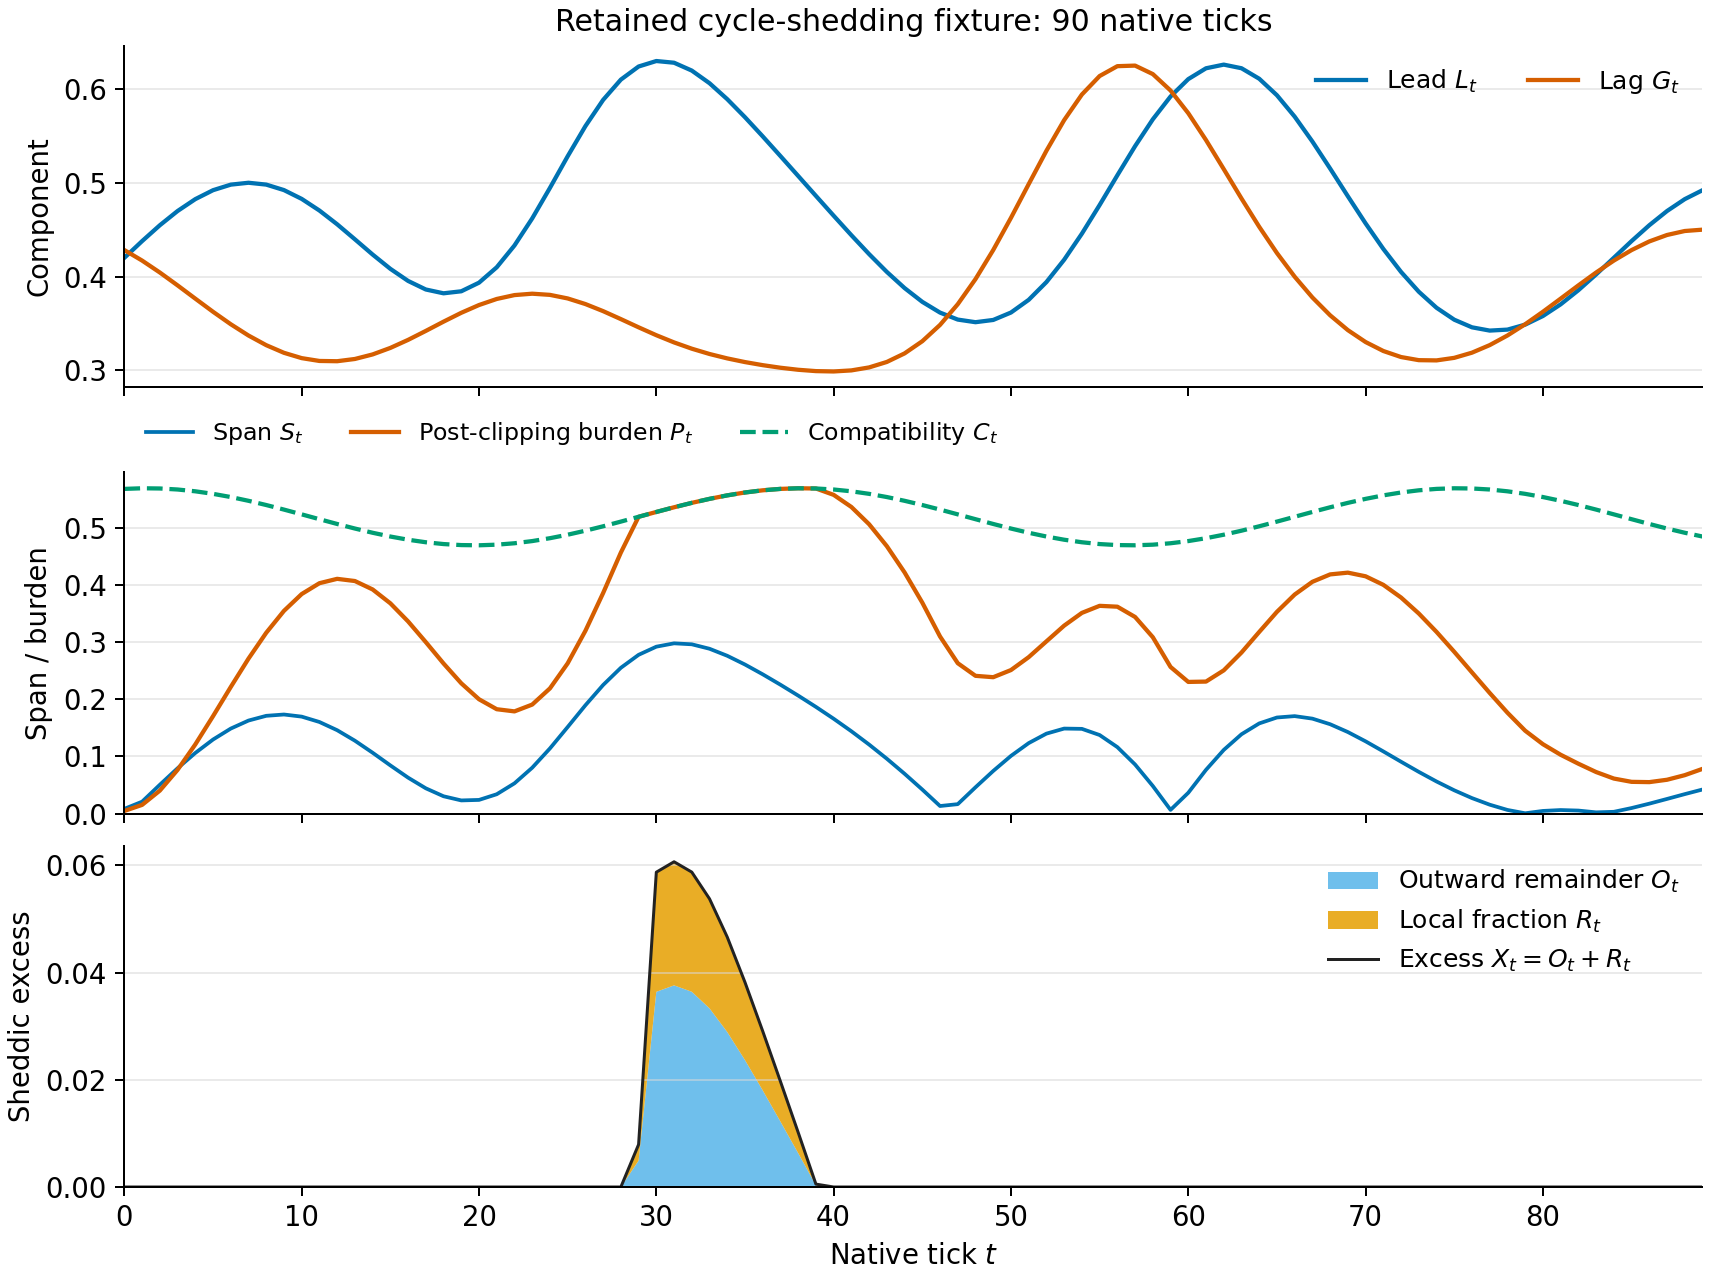
\includegraphics[width=0.98\linewidth]{../figures_jpg/cycle_disturbance_shedding_fixture.png}
\caption{Retained temporal-cycle fixture. The burden \(P_t\) is post-clipping, with \(P_t\le C_t\); the stacked outward and local fractions sum to \(X_t\). Figure and summary use the same CSV. The summary label ``Total exoshedding'' denotes \(\sum_t O_t\) in this fixture.}
\label{fig:v39-cycle-shedding-simulation}
\end{figure}

\begin{center}
\begin{tabular}{lr}
\toprule
Update steps & 90 \\
Maximum lead-lag span & 0.298 \\
Maximum temporal SADAR burden & 0.570 \\
Maximum sheddic excess & 0.061 \\
Total exoshedding & 0.238 \\
Total local reclosure & 0.146 \\
Sheddic path trigger updates & 0 \\
First reclosure update & none \\
\bottomrule
\end{tabular}

\end{center}

\subsection{Falsification}
\label{manual:cycle-shedding-run-verdict}
If the computed values violate the stated recurrences on the declared ticks, the demonstration fails on that run.

\subsection{Data-support class reference}\label{manual:app:data-support-class-reference}
Manual fixtures and comparisons are read together with their declared data-support class. The compact class list is:
\[
\begin{array}{c|l}
D0 & \text{exact internal fixture},\\
O0 & \text{observable-map fixture},\\
G0 & \text{radial shell projection},\\
G1 & \text{radial-medium projection},\\
G2 & \text{three-dimensional field-dynamics retention},\\
G3 & \text{time-resolved tracer-current simulation},\\
L0 & \text{exact lensing toy fixture},\\
L1 & \text{radial lens-medium diagnostic},\\
L2 & \text{target-acquisition lane},\\
L3 & \text{full lensing release class}.
\end{array}
\]
Errors and residuals are scoped to the class: \(\delta_3\) for exact internal comparators, observable-map residuals for O0, radial square-speed residuals for G0/G1, retention and field residuals for G2/G3, and target-side residuals for L2/L3 after prediction values freeze.

\subsection{Audit}\label{manual:simfix:falsification}
Fixture audit records signed direction, scalar pressure, scope cancellation inside its declared boundary/window, and \(\mathcal E(R,B)\) for a declared Stokes-valid scope.

\aodprovenance{\mainequation{main:eq:b-scoped-flux}; \mainequation{main:eq:sadar-attention-vector}; \mainequation{main:eq:stokes-audit-residual}; \mainappendix{main:app:symbolic-cancellation-check}; \mainappendix{main:app:combinatorics-rd-tests}.}

\subsection{Prediction-test placement}
Prediction tests and any collision-window comparison context belong in this manual scaffold. Application labels and external comparison records are carried by this manual scaffold. The main A\(\Omega\)D note supplies the AF/AFC/A\(\Omega\)D calculus and internal form names.
